%********************************************************************
% Appendix
%*******************************************************
% If problems with the headers: get headings in appendix etc. right
%\markboth{\spacedlowsmallcaps{Appendix}}{\spacedlowsmallcaps{Appendix}}
\chapter{Appendix}
\label{Appendix}

\begin{lstlisting}[language=C++,frame=tb,caption={Deployment und Service von Keycloak},label=lst:DeploymentundServicevonKeycloak]
    apiVersion: v1
    kind: Service
    metadata:
      name: keycloak
      labels:
        app: keycloak
    spec:
      ports:
      - name: http
        port: 9080
        targetPort: 9080
      selector:
        app: keycloak
      type: LoadBalancer
    ---
    apiVersion: apps/v1
    kind: Deployment
    metadata:
      name: keycloak
      namespace: default
      labels:
        app: keycloak
    spec:
      replicas: 1
      selector:
        matchLabels:
          app: keycloak
      template:
        metadata:
          labels:
            app: keycloak
        spec:
          containers:
          - name: keycloak
            image: quay.io/keycloak/keycloak:12.0.4
            env:
            - name: PROXY_ADDRESS_FORWARDING
              value: "true"
            - name: DB_VENDOR
              value: "postgres"
            # Der PostgreSQL Nutzer
            - name: DB_USER
              value: "postgres"
            # Das Passwort des PostgreSQL Nutzers
            - name: DB_PASSWORD
              value: "postgrespw"
            # Die Adresse der PostgreSQL-Datenbank in der Notation: "<postgres-service-name>"."<namespace>"
            - name: DB_ADDR
              value: "postgres-db-lb.default"
            # Name der PostgreSQL Datenbank, in der Keycloak-Einstellungen gespeichert werden
            - name: DB_DATABASE
              value: "postgres"
            # Name des Keycloak Nutzers
            - name: KEYCLOAK_USER
              value: "admin"
            # Passwort des Keycloak Nutzers
            - name: KEYCLOAK_PASSWORD
              value: "admin"
            ports:
            - name: http
              containerPort: 9080
            - name: https
              containerPort: 9443
            args:
            - "-Djboss.socket.binding.port-offset=1000"
            readinessProbe:
              httpGet:
                path: /auth/realms/master
                port: 9080    
  \end{lstlisting}
  \bigskip

  \begin{lstlisting}[language=C++,frame=tb,caption={Deployment und Service von PostgreSQL als Datenbank für Keycloak},label=lst:DeploymentundServicevonPostgres]
    # PostgreSQL StatefulSet
    apiVersion: apps/v1
    kind: StatefulSet
    metadata:
      name: postgresql-db
    spec:
      serviceName: postgresql-db-service
      selector:
        matchLabels:
          app: postgresql-db
      replicas: 1
      template:
        metadata:
          labels:
            app: postgresql-db
        spec:
          containers:
            - name: postgresql-db
              image: postgres:13.4
              volumeMounts:
                - name: postgresql-db-disk
                  mountPath: /data
              env:
                - name: POSTGRES_DATABASE
                  value: "postgres"
                - name: POSTGRES_PASSWORD
                  value: "postgrespw"
                - name: PGDATA
                  value: /data/pgdata
      # Volume Claim
      volumeClaimTemplates:
        - metadata:
            name: postgresql-db-disk
          spec:
            accessModes: ["ReadWriteOnce"]
            resources:
              requests:
                storage: 1Gi
    ---
    # PostgreSQL StatefulSet Service
    apiVersion: v1
    kind: Service
    metadata:
      name: postgres-db-lb
    spec:
      selector:
        app: postgresql-db
      type: LoadBalancer
      ports:
        - port: 5432
          targetPort: 5432            
  \end{lstlisting}
  \bigskip

  \begin{figure}[H]
    \centering
    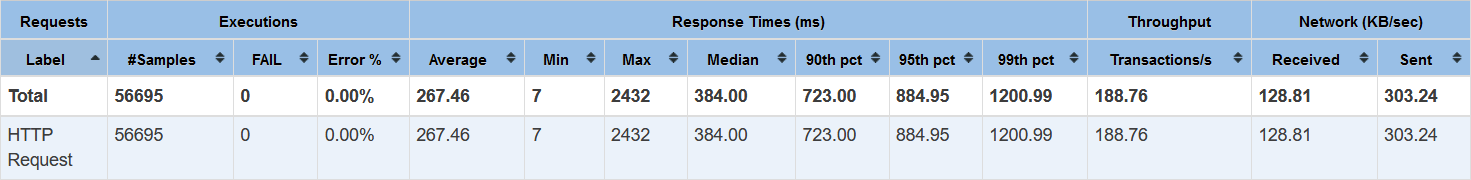
\includegraphics[width=1.0\textwidth]{gfx/statistik-skalierung-opa-k8s.png}
    \caption{Statistiken von Skalierbarkeitstest von Ressource Server mit OPA in einem Kubernetes Cluster}
    \label{fig:chapter04:statistik-skalierung-opa-k8s}
  \end{figure}

  \begin{figure}[H]
    \centering
    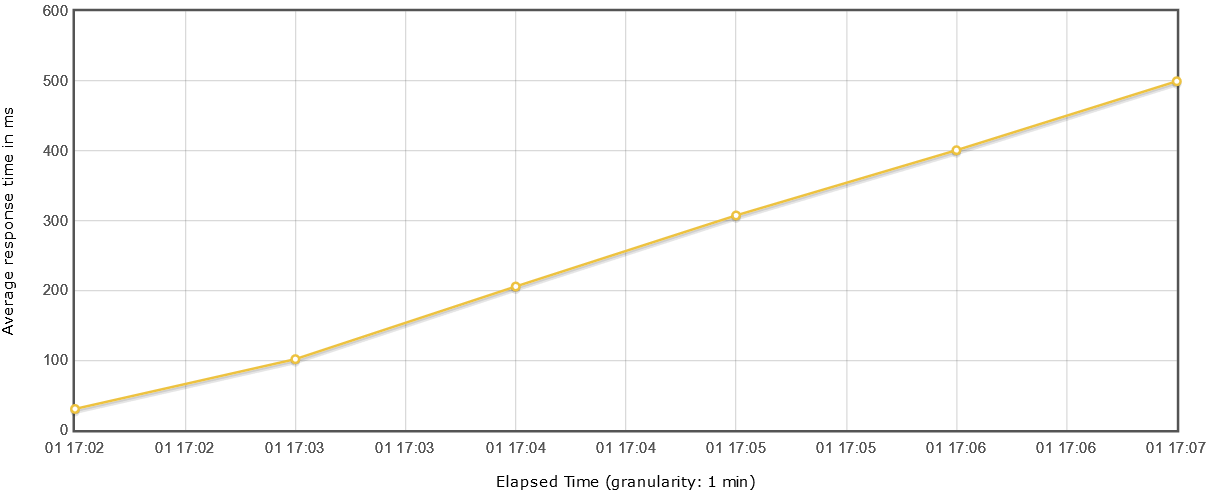
\includegraphics[width=1.0\textwidth]{gfx/flotResponseTimesOverTime-skalierung-opa-k8s.png}
    \caption{Response Time Graph von Skalierbarkeitstest von Ressource Server mit OPA in einem Kubernetes Cluster}
    \label{fig:chapter04:flotResponseTimesOverTime-skalierung-opa-k8s}
  \end{figure}

  \begin{figure}[H]
    \centering
    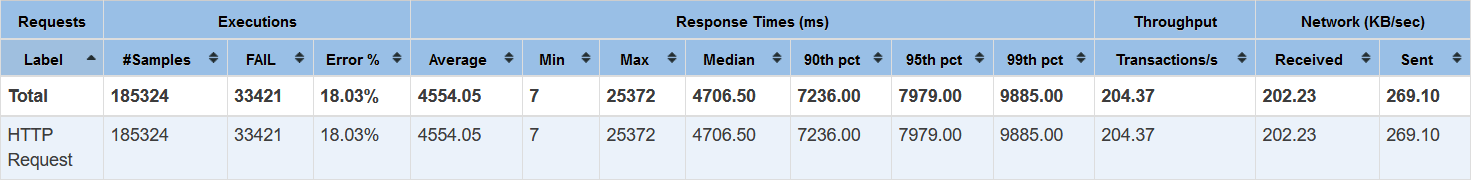
\includegraphics[width=1.0\textwidth]{gfx/statistik-stress-opa-k8s.png}
    \caption{Statistiken von Stresstest von Ressource Server mit OPA in einem Kubernetes Cluster}
    \label{fig:chapter04:statistik-stress-opa-k8s}
  \end{figure}